\documentclass[11pt,a4paper]{article}
\usepackage[utf8]{inputenc}
\usepackage[T1]{fontenc}
\usepackage[romanian]{babel}
\usepackage[margin=2cm]{geometry}
\usepackage{array}
\usepackage{tabularx}
\usepackage{enumitem}
\usepackage{graphicx}
\usepackage{setspace}
\usepackage{xcolor}
\usepackage{hyperref}
\usepackage{amssymb}
\setlength{\parindent}{0pt}
\newcommand{\fillline}[1][6cm]{\underline{\hspace{#1}}}
\newcommand{\fillbox}[1][0.4cm]{\framebox[#1]{\rule{0pt}{#1}}}
\newcommand{\checkboxempty}{$\square$}

\begin{document}

\noindent
\begin{minipage}[t]{0.40\textwidth}
\vspace{0pt}
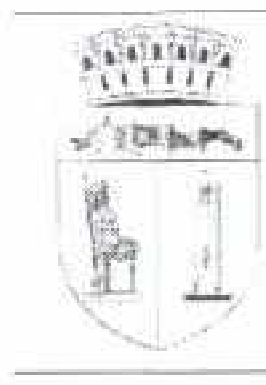
\includegraphics[height=1.5cm]{../assets/stema-cluj.png}%
\hspace{0.2cm}%
\raisebox{0.5cm}{\parbox[t]{3.5cm}{\textbf{PRIMĂRIA}\\\textbf{CLUJ-NAPOCA}}}
\end{minipage}%
\begin{minipage}[t]{0.30\textwidth}
\centering
\vspace{0.4cm}

\includegraphics[width=3.5cm,height=0.9cm]{../assets/barcode-460007.png}
\end{minipage}%
\begin{minipage}[t]{0.30\textwidth}
\raggedleft
\vspace{0.6cm}
Nr. \fillline[3cm] / \fillline[1cm]
\end{minipage}

\vspace{0.3cm}
\hrule
\vspace{0.5cm}

\begin{center}
\textbf{CĂTRE,}\\
\textbf{DIRECŢIA ECOLOGIE URBANĂ ŞI SPAŢII VERZI}\\
\textbf{SERVICIUL SPAŢII VERZI}
\end{center}

\vspace{0.4cm}

\begin{center}
\textbf{C E R E R E}\\
\textit{pentru eliberarea} \textbf{AVIZULUI pentru doborâre arbori din curți private}
\end{center}

\vspace{0.8cm}

\hspace{1cm}SUBSEMNATUL/SUBSCRISA \fillline[10cm]

\vspace{0.3cm}

\hspace{1cm}ADRESA/SEDIUL \fillline[12cm]

\vspace{0.3cm}

\hspace{1cm}TELEFON \fillline[13cm]

\vspace{0.6cm}

\hspace{1cm}Solicit eliberarea AVIZULUI pentru doborârea unui număr de \fillline[1.5cm] arbori

pe strada \fillline[8cm] nr. \fillline[5cm]

\vspace{0.5cm}

Documentele necesare pentru eliberarea AVIZULUI care se vor anexa prezentei cereri:

\vspace{0.3cm}

\textbf{A. PIESE SCRISE:}

\vspace{0.3cm}

\begin{enumerate}[leftmargin=2cm]
\item Copie după Extrasul de Carte Funciară (nu mai vechi de 3 luni)
\item Document fotografic pentru fiecare arbore în parte
\item CUPON DE PENSIE (unde este cazul)
\end{enumerate}

\vspace{0.5cm}

\checkboxempty\ Prin prezenta solicit comunicarea răspunsului pe următoarea adresă de e-mail:

\vspace{0.2cm}

\fillline[14cm]

\vspace{0.4cm}

\checkboxempty\ Mă oblig să comunic instituției orice modificare intervine în legătură cu această adresă de e-mail

\checkboxempty\ Îmi exprim consimțământul ca Primăria Municipiului Cluj-Napoca să comunice orice informații, date personale, clarificări și completări pe adresa de e-mail indicată mai sus.

\checkboxempty\ Am luat la cunoștință faptul că în cazul nefuncționării serverului de e-mail comunicat sau în cazul adresei greșite de e-mail, Municipiul Cluj-Napoca nu poate fi tras la răspundere pentru acest lucru.

\vspace{0.8cm}

\hspace{1cm}Data \hfill Semnătură \dotfill (persoană, președinte/administrator)\hspace{1cm}

\vspace{0.2cm}

\hspace{1cm}\fillline[5cm] \hfill (CUI \dotfill )\hspace{1cm}

\vfill
\hrule
\vspace{0.3cm}

\begin{minipage}[t]{0.65\textwidth}
www.primariaclujnapoca.ro\\
telefon: 0264/596.030\\
Cluj-Napoca, str. Moţilor, nr. 3
\end{minipage}%
\begin{minipage}[t]{0.35\textwidth}
\raggedleft

\includegraphics[width=3cm,height=0.7cm]{../assets/barcode-460007.png}
\end{minipage}

\vspace{0.3cm}
\hrule
\vspace{0.2cm}

{\footnotesize
\textbf{Timp estimativ de completare: 10 minute}

\vspace{0.2cm}

Datele personale care vă sunt solicitate prin prezenta cerere vor fi prelucrate numai în vederea procesării și soluționării solicitării dumneavoastră. Primăria municipiului Cluj-Napoca garantează securitatea procesării datelor și arhivarea acestora în conformitate cu prevederile legale în vigoare. Responsabilul Primăriei municipiului Cluj-Napoca cu protecția datelor poate fi contactat pe adresa de email dpo@primariaclujnapoca.ro.

\vspace{0.2cm}

În conformitate cu Regulamentul nr. 679/2016 aveți dreptul de a solicita Primăriei municipiului Cluj-Napoca, în ceea ce priveşte datele cu caracter personal referitoare la persoana vizată, accesul la acestea, rectificarea sau ştergerea acestora sau restricţionarea prelucrării sau a dreptului de a vă opune prelucrării, precum şi a dreptului la portabilitatea datelor.
}

\end{document}
